\section{实证评估}
\label{sec:experiments}

我们评估\faf相对于各种开源和闭源基线的效率。

\paragraph{注意力基准测试。}我们在不同序列长度和头维度下测量\faf的运行时间，将其与PyTorch标准实现、\faa\footnote{\fat不支持B200}、Triton（使用特定于B200的指令~\citep{tillet2019triton}）、Gluon（一种比Triton具有更精细控制的底层GPU编程语言~\citep{gluon2024}）以及cuDNN（针对B200 GPU优化的厂商库）进行比较。我们确认\faf比cuDNN 9.13最高快1.3倍，比Triton最高快2.7倍。\faf在B200 GPU上达到最高1613 TFLOPS/s，约为理论最大TFLOPS/s的71\%。

\paragraph{基准测试设置。}我们在B200 GPU上针对不同设置（是否使用因果掩码，头维度64、128和(192, 128)）对BF16输入测量运行时间。序列长度从1k、2k、...至32k，批次大小设置为总token数为32k。隐藏维度设为2048，头维度为64或128（即32个头或16个头）。对于DeepSeek V3~\citep{deepseekai2024deepseekv3technicalreport}使用的(192, 128)配置，我们使用16个头，查询维度为192，键值维度为128。前向传播的FLOP计算公式为$4 \cdot \text{seqlen}^2 \cdot \text{head dimension} \cdot \text{number of heads}$。
对于因果掩码，我们将此数除以2，以考虑大约只有一半条目被计算的事实。后向传播的FLOP通过将前向传播FLOP乘以2.5得到（因为前向传播有2次矩阵乘法，后向传播有5次，由于重新计算）。

\subsection{前向传播}

\begin{figure*}[t]
  \centering
  \begin{minipage}{0.48\textwidth}
    \centering
    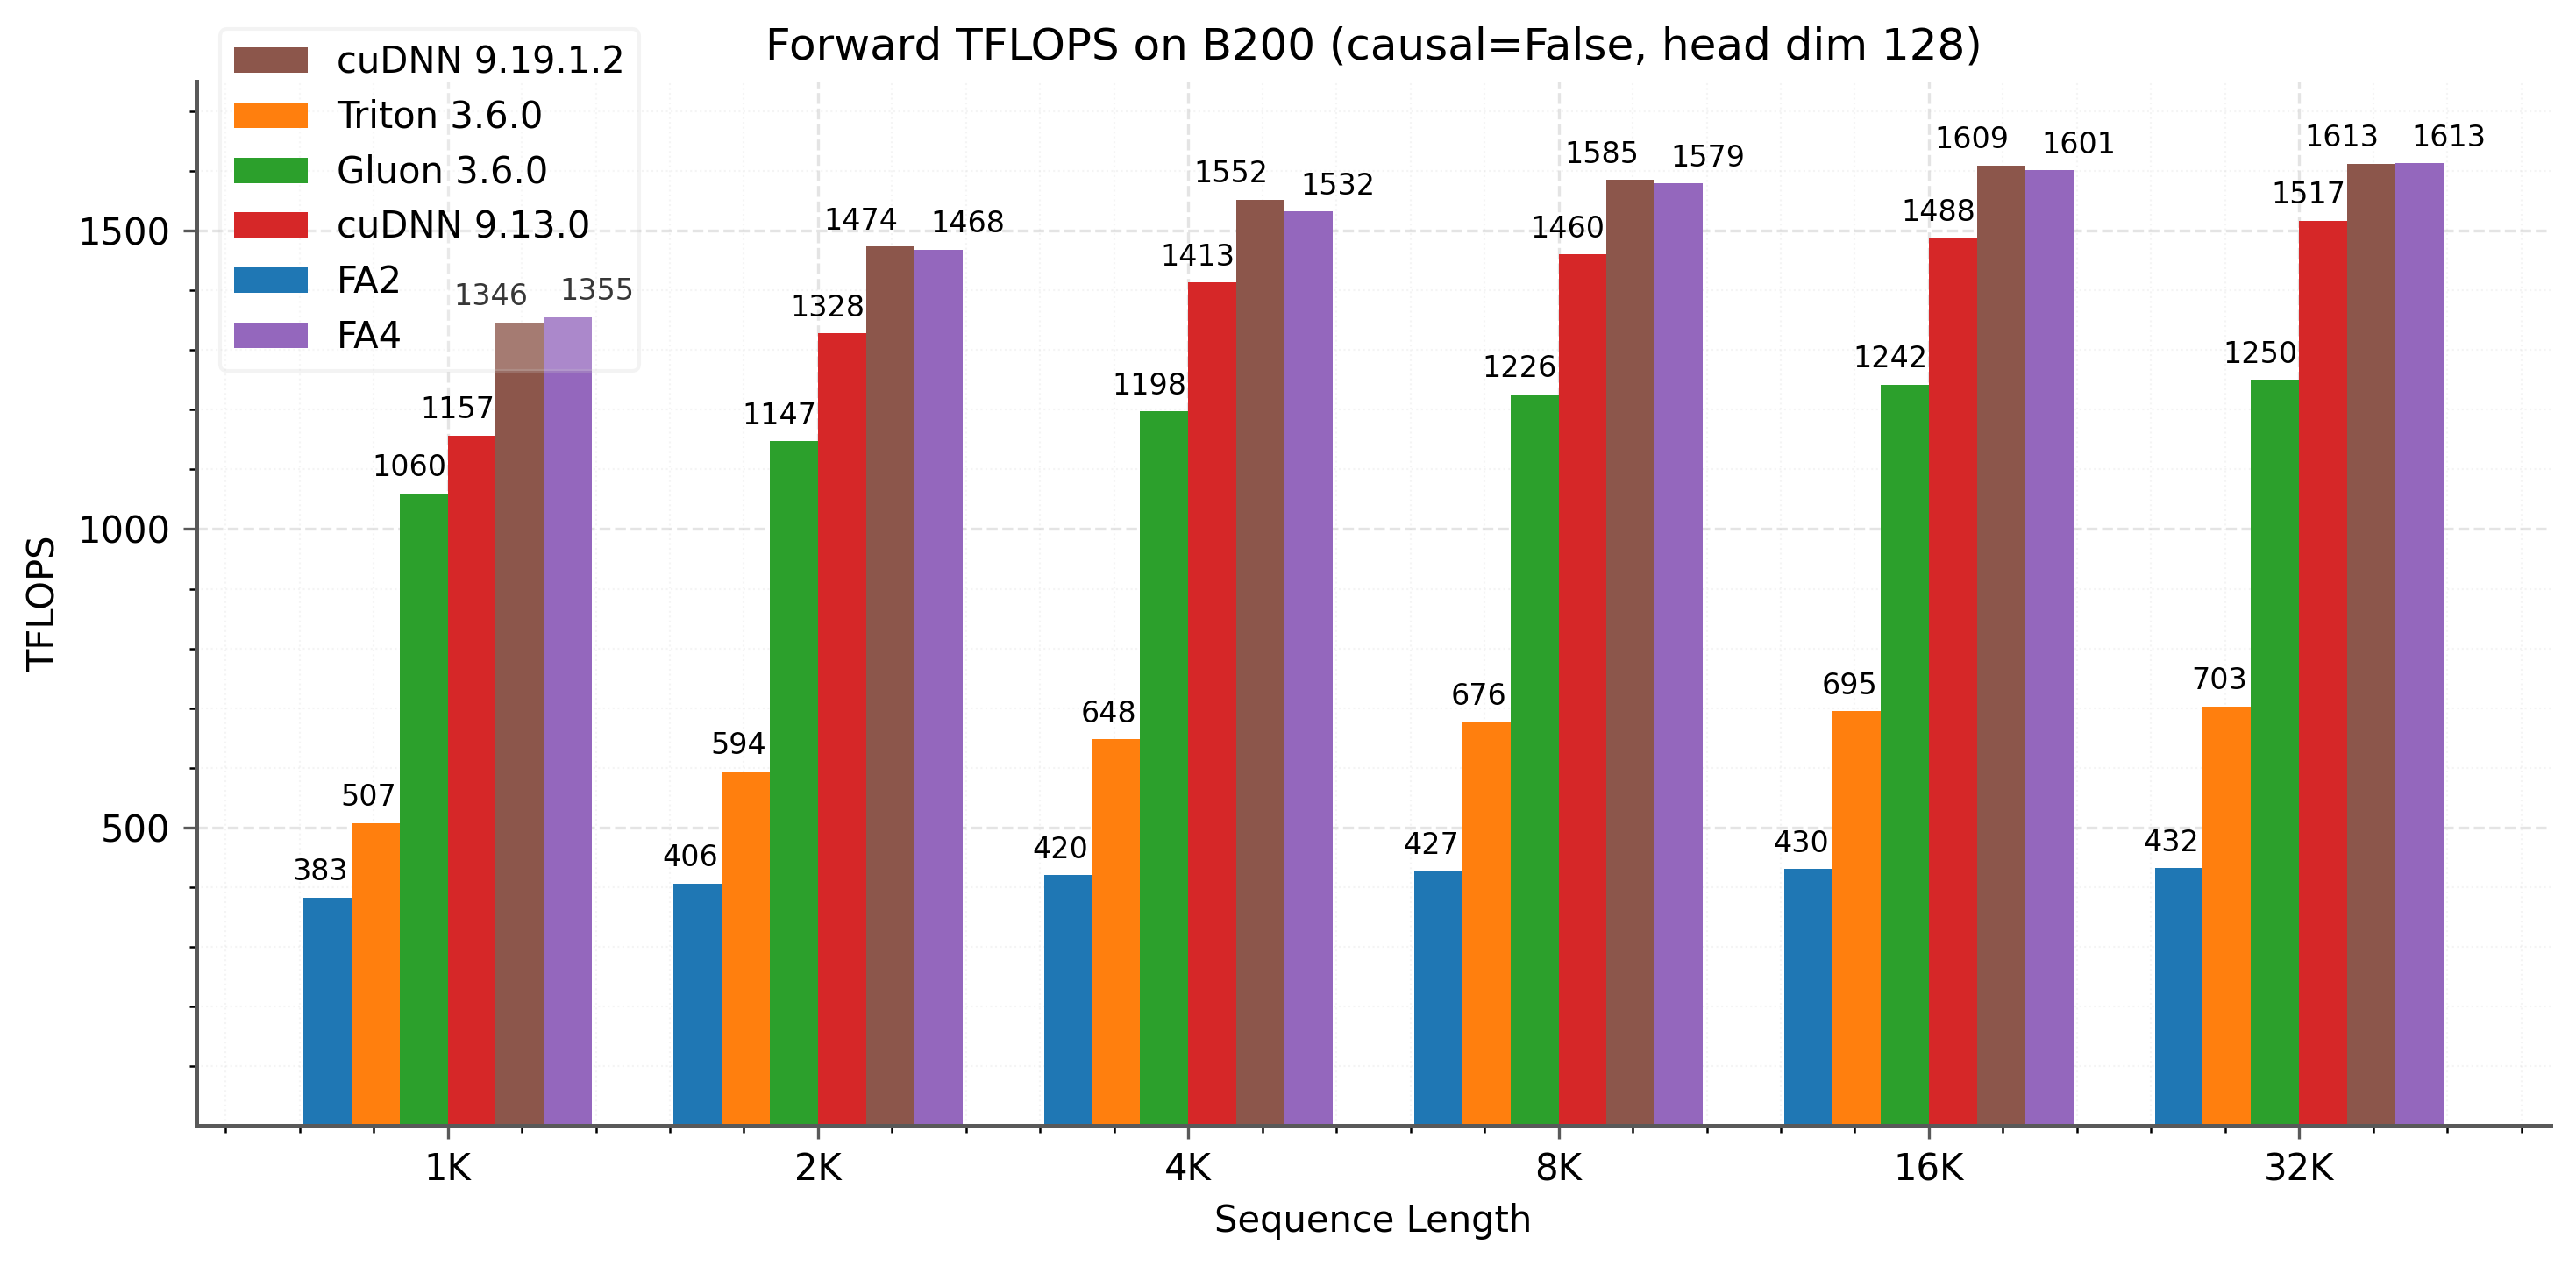
\includegraphics[width=\textwidth]{../Figures/fa4_fwd_causalFalse_hdim128_updated.png}
  \end{minipage}
  \hfill
  \begin{minipage}{0.48\textwidth}
    \centering
    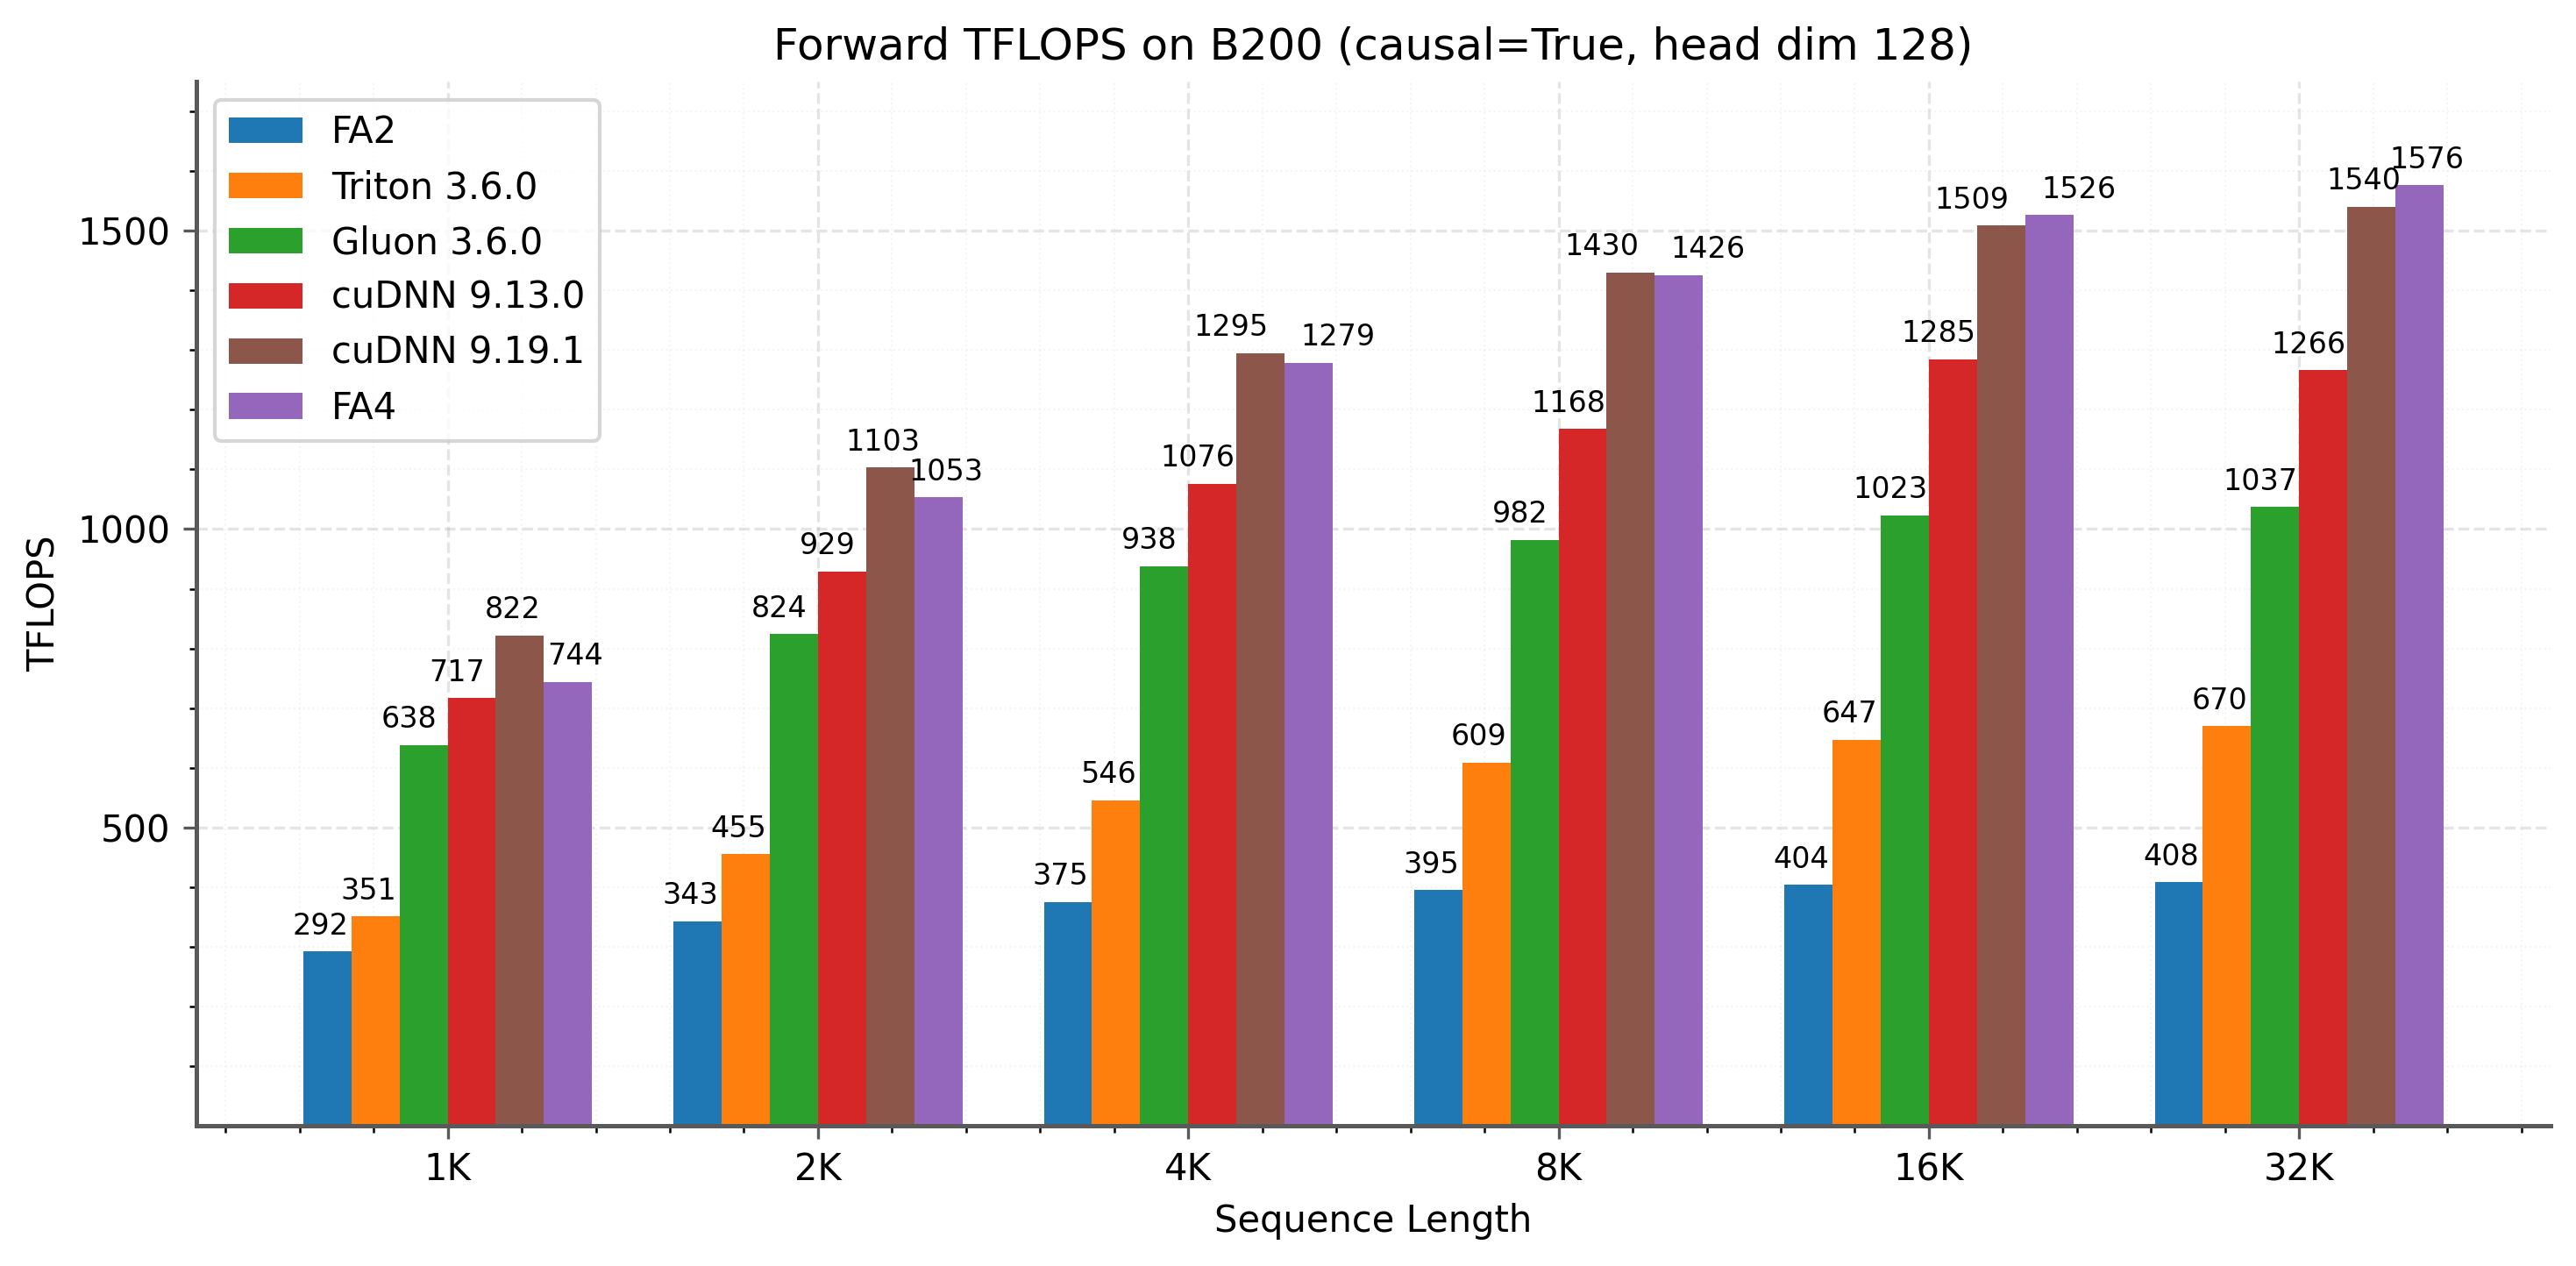
\includegraphics[width=\textwidth]{../Figures/fa4_fwd_causalTrue_hdim128_updated.png}
  \end{minipage}
\caption{B200（FP16/BF16）前向传播TFLOPS，头维度128。左：非因果注意力。右：因果注意力。在各序列长度上，FA4比cuDNN 9.13.0实现1.1--1.3倍加速，比Triton实现2.1--2.7倍加速。自我们实现的初始发布以来，cuDNN的新版本已纳入本文描述的许多技术，性能与FA4相近。}
  \label{fig:fwd}
\end{figure*}

我们在图~\ref{fig:fwd,fig:fwd_hdim192128}中报告前向传播结果，显示\faf比cuDNN 9.13快1.1--1.3倍，比Triton快2.1--2.7倍。对于中等和长序列（4k及以上），\faf在不同头维度和因果掩码设置下一致地优于所有基线。
因果情况下的提升更大，我们将其归因于最长处理时间优先（LPT）调度器。

\begin{figure}[h]
  \centering
  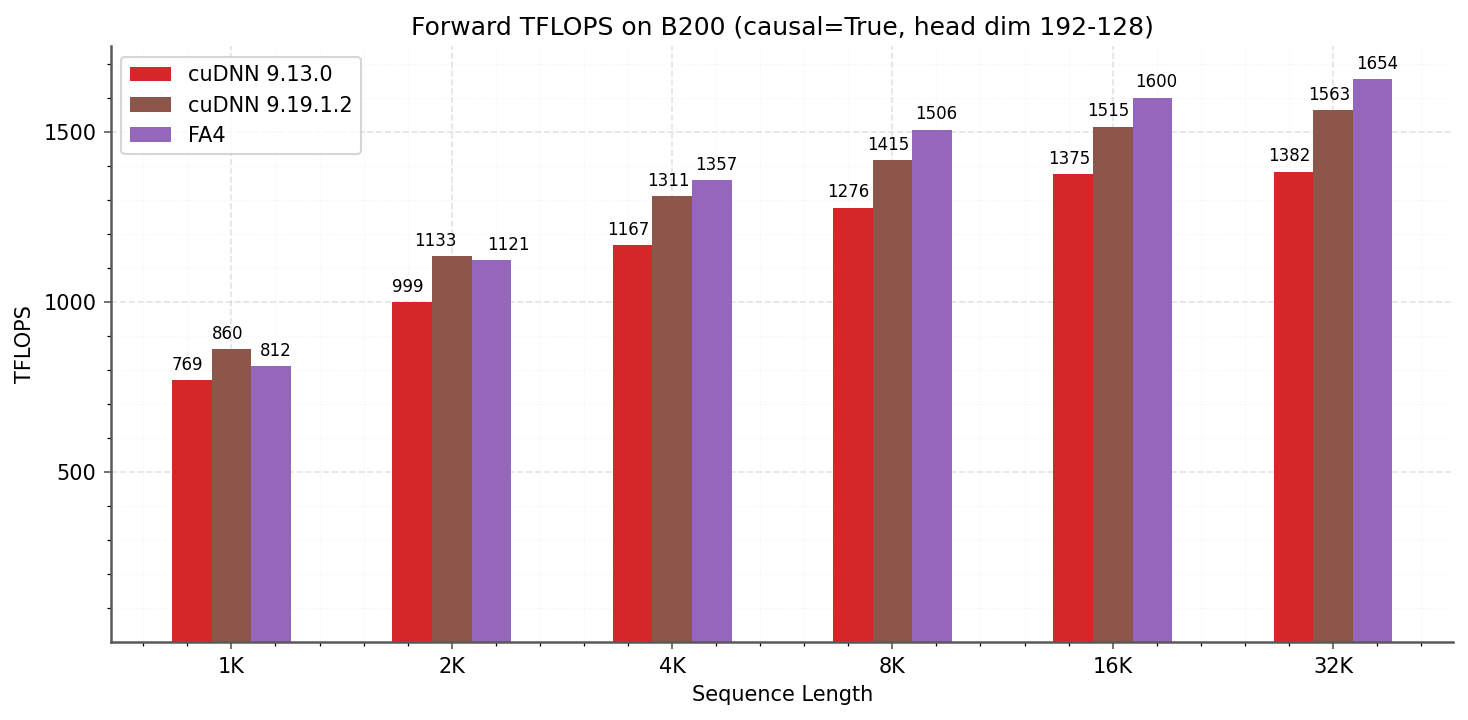
\includegraphics[width=0.65\columnwidth]{../Figures/fa4_fwd_causalTrue_hdim192128_updated.png}
  \caption{B200（FP16/BF16）因果注意力下cuDNN与FA4前向传播TFLOPS比较，头维度(192, 128)（DeepSeek V3架构中常用）}
  \label{fig:fwd_hdim192128}
\end{figure}

\subsection{后向传播}

\begin{figure*}[t]
  \centering
  \begin{minipage}{0.48\textwidth}
    \centering
    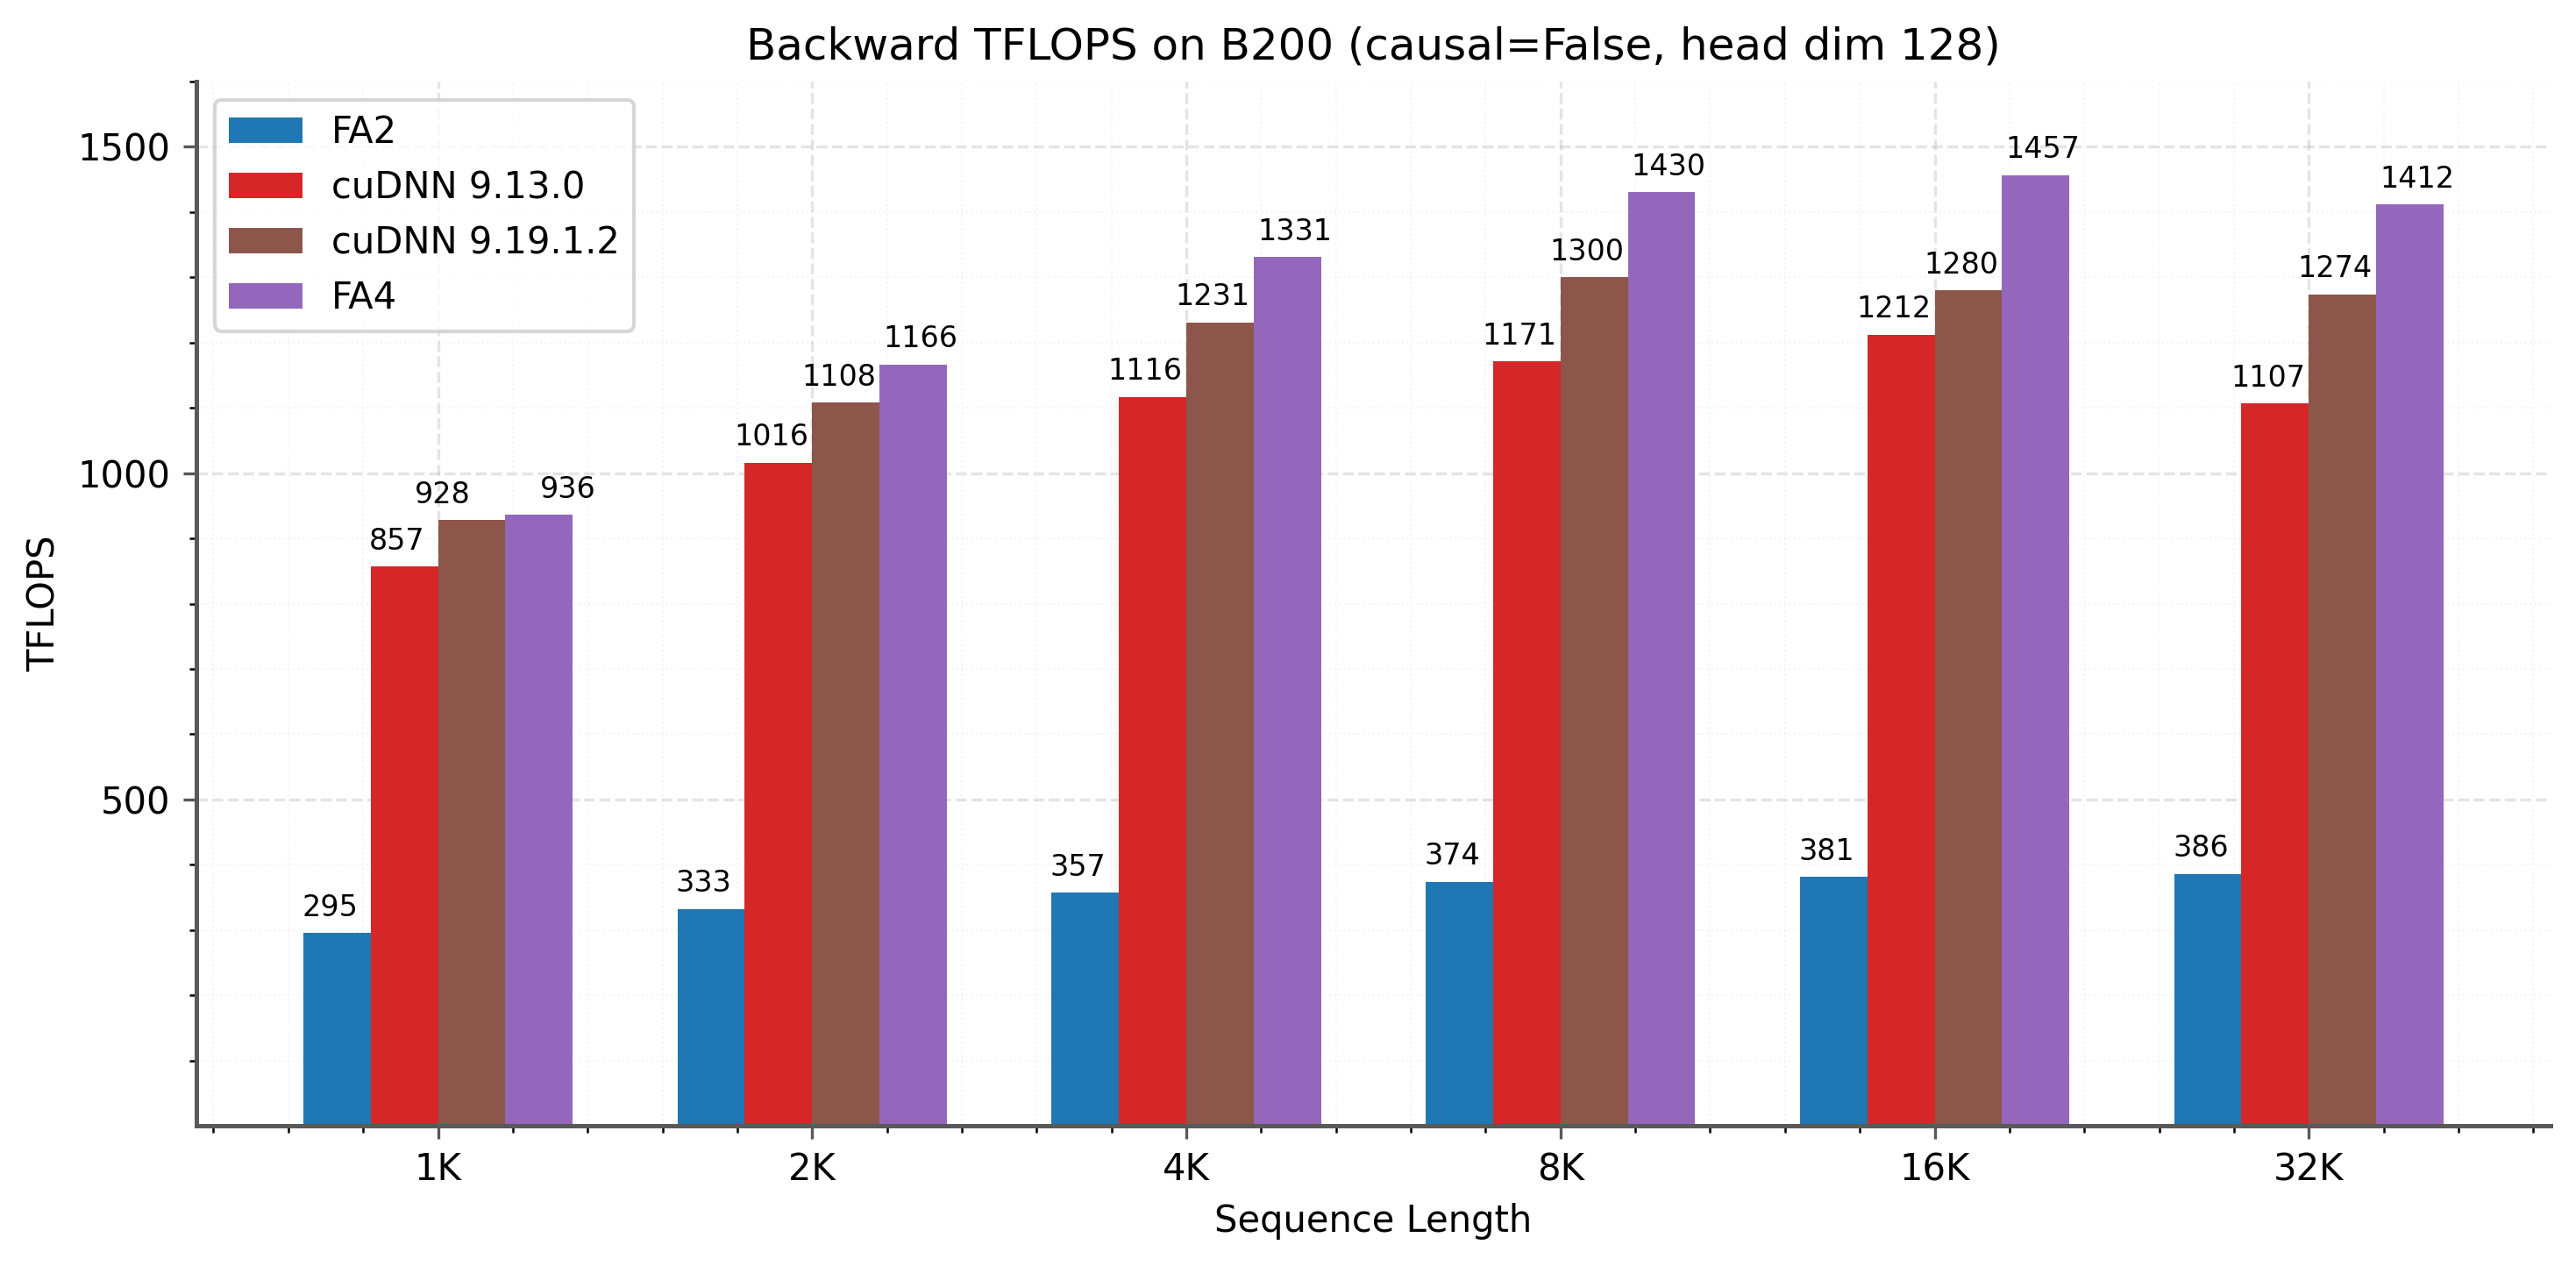
\includegraphics[width=\textwidth]{../Figures/fa4_bwd_causalFalse_hdim128_updated.png}
  \end{minipage}
  \hfill
  \begin{minipage}{0.48\textwidth}
    \centering
    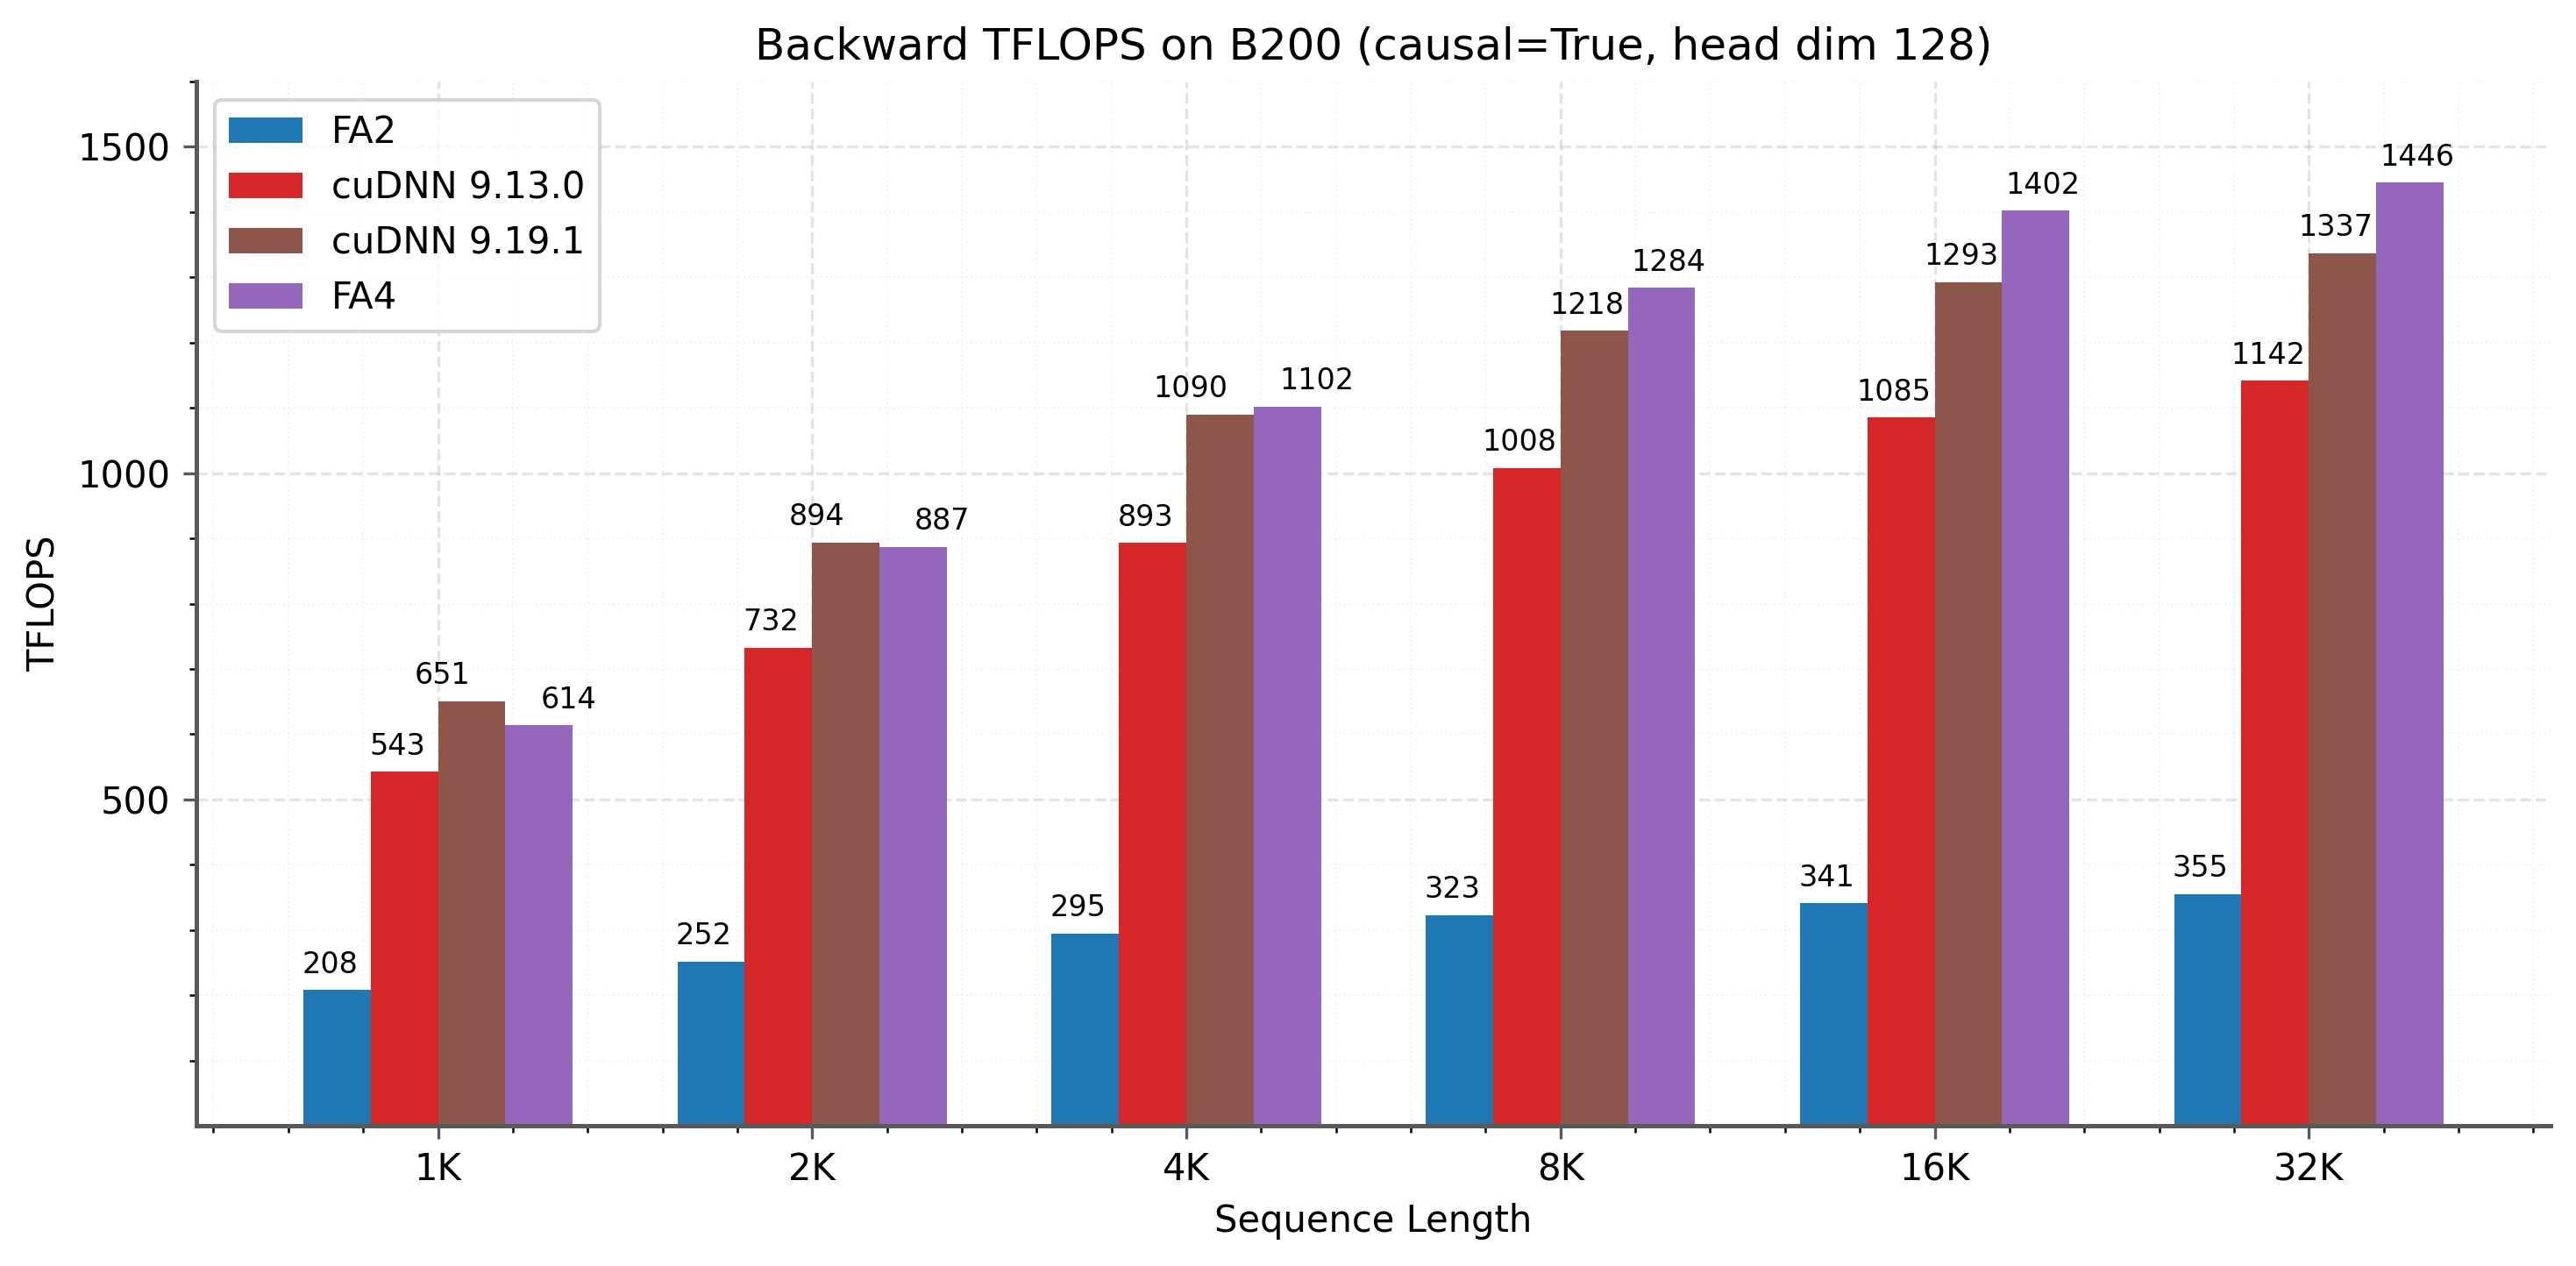
\includegraphics[width=\textwidth]{../Figures/fa4_bwd_causalTrue_hdim128_updated.png}
  \end{minipage}
  \caption{B200（FP16/BF16）后向传播TFLOPS，头维度128。左：非因果注意力。右：因果注意力。}
  \label{fig:bwd}
\end{figure*}

我们在图~\ref{fig:bwd}中报告后向传播结果。\faf在长序列和因果掩码下实现了一致的加速，证明了我们2-CTA后向传播的有效性。

我们还在图~\ref{fig:bwd-det-ablation}中展示了确定性后向传播的性能。我们精心设计的数据重排和调度使确定性后向传播速度大幅提升，达到1-CTA非确定性后向传播速度的75\%。

\begin{figure}[h]
  \centering
  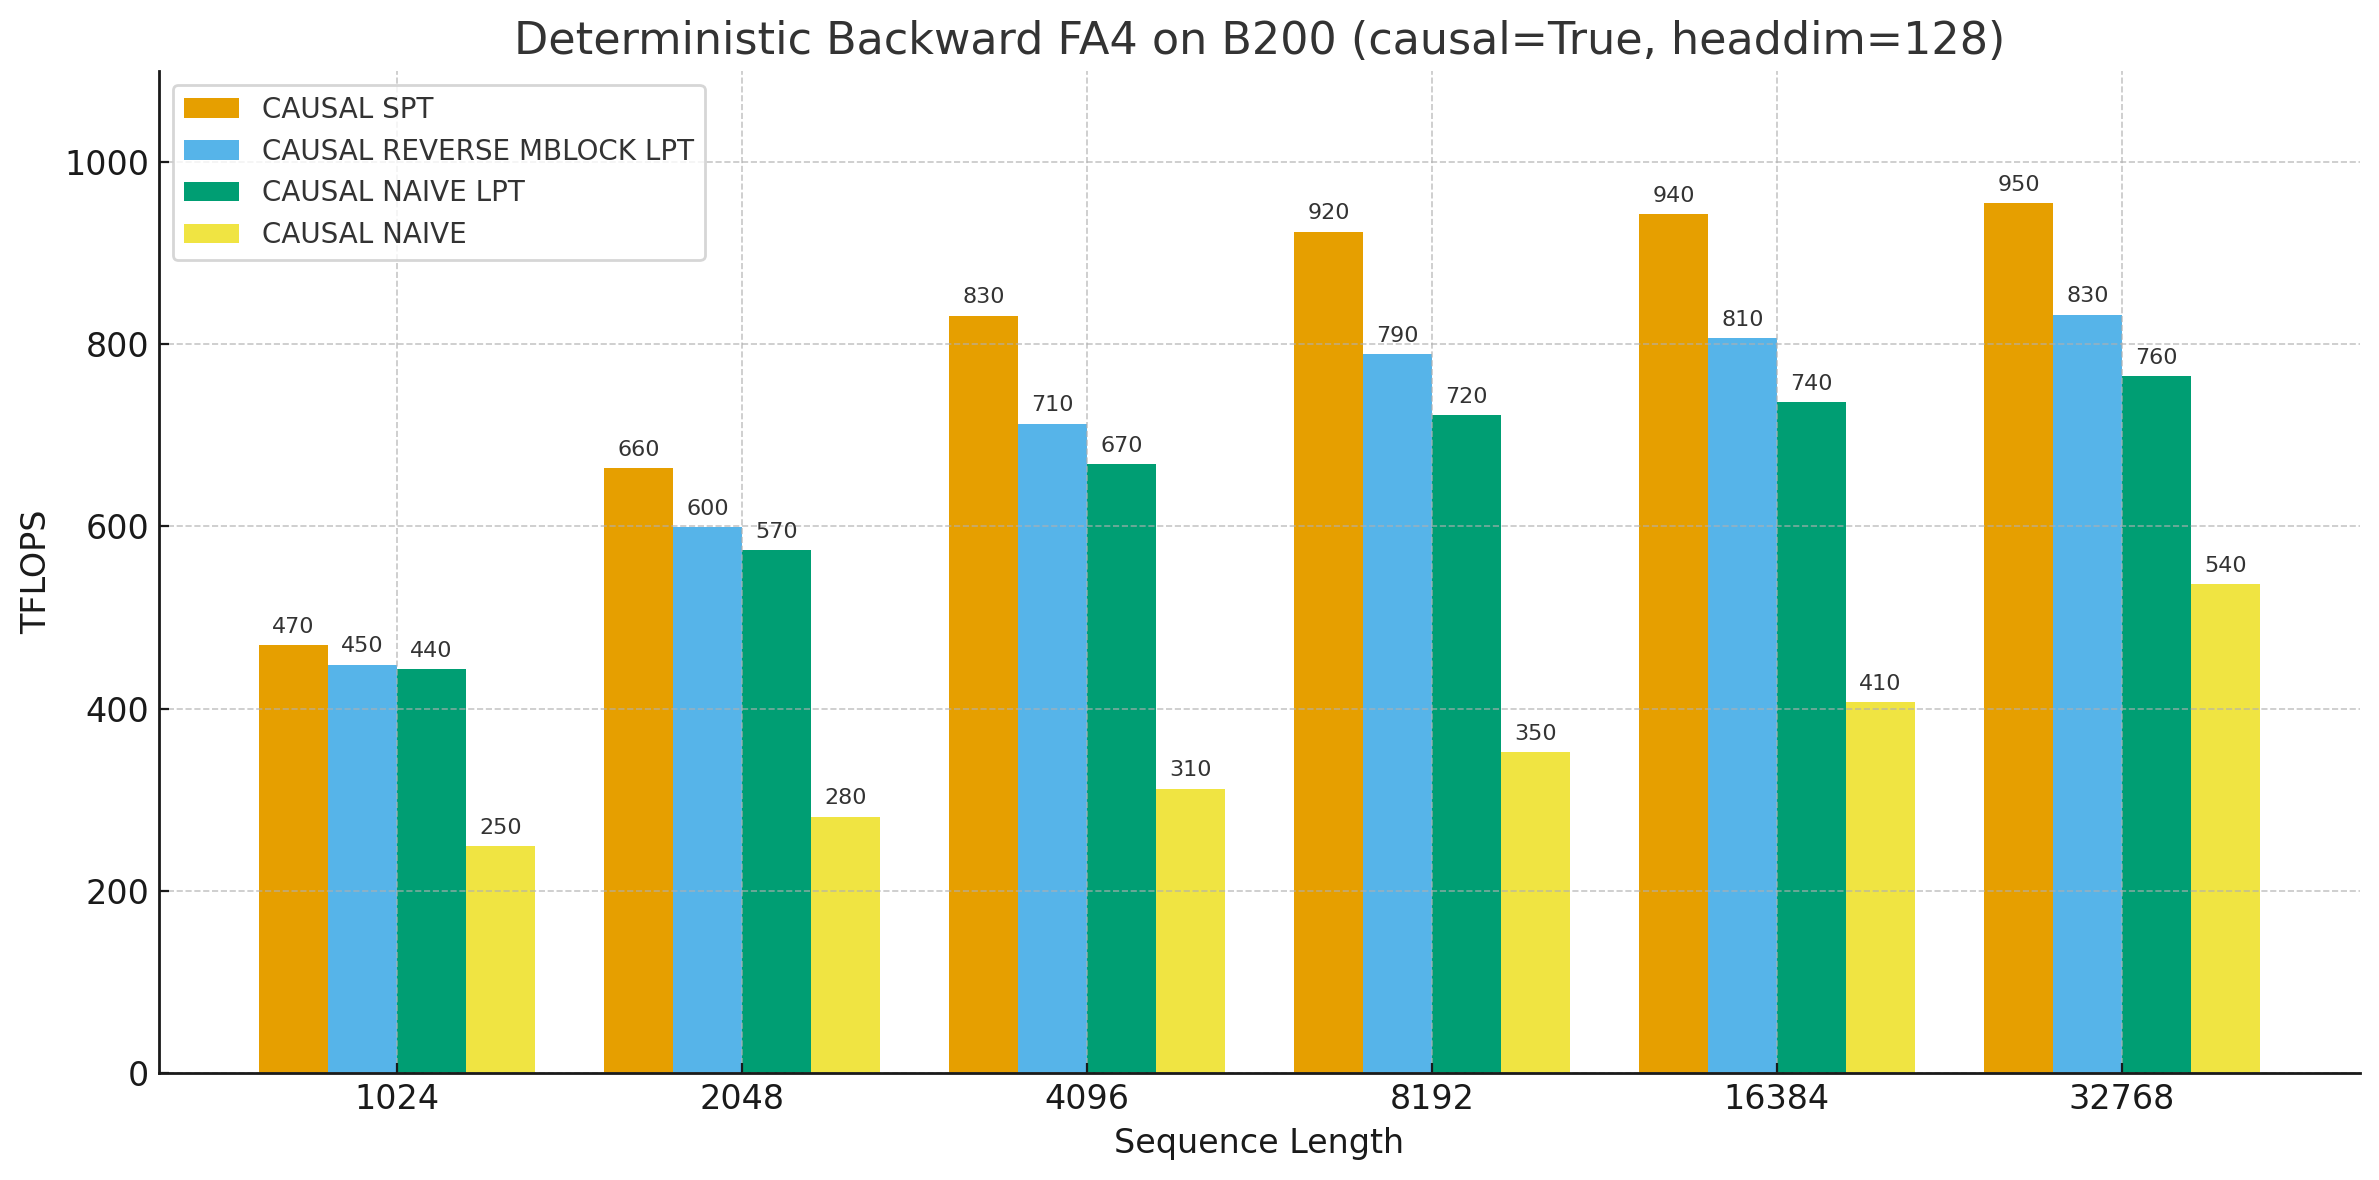
\includegraphics[width=0.95\columnwidth]{../Figures/causal_bwd_det_FA4.png}
  \caption{B200（FP16/BF16）确定性后向传播消融实验，头维度128。因果注意力——SPT、逆序m块的LPT、LPT以及无批次/头重排的朴素方法。}
  \label{fig:bwd-det-ablation}
\end{figure}
